% 第2章：原书印刷页5--16，按原文逐页重译；公式及算法均为可编辑原生内容。
\sourcepage{5}
所有非线性优化方法都是迭代方法：从起始点 $\mathbf{x}_0$ 出发，方法产生一列向量
$\mathbf{x}_1,\mathbf{x}_2,\ldots$，它们（希望能够）收敛到给定函数的一个局部极小点
$\mathbf{x}^{\ast}$，见定义~1.3。大多数方法都采取措施，强制满足\emph{下降条件}
\begin{equation}
  F(\mathbf{x}_{k+1})<F(\mathbf{x}_k).
  \tag{2.1}\label{eq:2.1}
\end{equation}
这可以防止迭代收敛到极大点，也降低了收敛到鞍点的可能性。如果给定函数有多个极小点，
结果就取决于起始点 $\mathbf{x}_0$。我们不知道会找到其中的哪一个；它不一定是离
$\mathbf{x}_0$ 最近的极小点。

在许多情况下，方法产生的向量经过两个明显不同的阶段收敛到极小点。当 $\mathbf{x}_0$
远离解时，我们希望方法产生的迭代点稳步向 $\mathbf{x}^{\ast}$ 移动。在迭代的这一
“全局阶段”，只要除了最初几步以外误差不再增大，我们就可以满意，即
\[
  \norm{\mathbf{e}_{k+1}}<\norm{\mathbf{e}_k}\qquad\text{当 }k>K,
\]
其中 $\mathbf{e}_k$ 表示当前误差，
\begin{equation}
  \mathbf{e}_k=\mathbf{x}_k-\mathbf{x}^{\ast}.
  \tag{2.2}\label{eq:2.2}
\end{equation}

在迭代的最后阶段，$\mathbf{x}_k$ 已接近 $\mathbf{x}^{\ast}$，我们希望收敛得更快。
我们区分以下几种情形：

\emph{线性收敛：}
\begin{equation}
  \norm{\mathbf{e}_{k+1}}\leq a\norm{\mathbf{e}_k}
  \qquad\text{当 }\norm{\mathbf{e}_k}\text{ 较小时；}\quad 0<a<1,
  \tag{2.3a}\label{eq:2.3a}
\end{equation}

\sourcepage{6}
\emph{二次收敛：}
\begin{equation}
  \norm{\mathbf{e}_{k+1}}=O\bigl(\norm{\mathbf{e}_k}^{2}\bigr)
  \qquad\text{当 }\norm{\mathbf{e}_k}\text{ 较小时},
  \tag{2.3b}\label{eq:2.3b}
\end{equation}

\emph{超线性收敛：}
\begin{equation}
  \norm{\mathbf{e}_{k+1}}/\norm{\mathbf{e}_k}\longrightarrow0
  \qquad\text{当 }k\longrightarrow\infty.
  \tag{2.3c}\label{eq:2.3c}
\end{equation}

本讲义介绍的方法都是下降法，在每一步迭代中都满足下降条件~(2.1)。从当前迭代点
出发的一步包括：
\begin{enumerate}[label=\arabic*.,leftmargin=2em]
  \item 找到一个下降方向 $\mathbf{h}_{\mathrm d}$（下文讨论）；
  \item 找到一个步长，使 $F$ 值有较大的下降。
\end{enumerate}
因此，下降法的轮廓如下。

\needspace{16\baselineskip}
\begin{algorithmbox}{2.4}{下降法}
\begin{tabbing}
\hspace{1.3em}\=\hspace{1.3em}\=\hspace{1.3em}\=\hspace{1.3em}\=\kill
\textbf{begin}\\
\> $k:=0;\quad\mathbf{x}:=\mathbf{x}_0;\quad\mathit{found}:=\mathrm{false}$
   \quad\{起始点\}\\
\> \textbf{while} $(\textbf{not }\mathit{found})\ \textbf{and}\ (k<k_{\max})$\\
\>\> $\mathbf{h}_{\mathrm d}:=\text{搜索方向}(\mathbf{x})$
   \quad\{从 $\mathbf{x}$ 出发，沿下降方向\}\\
\>\> \textbf{if} （不存在这样的 $\mathbf{h}$）\\
\>\>\> $\mathit{found}:=\mathrm{true}$\quad\{$\mathbf{x}$ 是驻点\}\\
\>\> \textbf{else}\\
\>\>\> $\alpha:=\text{步长}(\mathbf{x},\mathbf{h}_{\mathrm d})$
   \quad\{从 $\mathbf{x}$ 出发，沿 $\mathbf{h}_{\mathrm d}$ 方向\}\\
\>\>\> $\mathbf{x}:=\mathbf{x}+\alpha\mathbf{h}_{\mathrm d};\quad k:=k+1$
   \quad\{下一个迭代点\}\\
\textbf{end}
\end{tabbing}
\end{algorithmbox}

考虑 $F$ 值沿着从 $\mathbf{x}$ 出发、方向为 $\mathbf{h}$ 的射线如何变化。由泰勒展开式~(1.4a)
可知
\begin{equation}
\begin{aligned}
  F(\mathbf{x}+\alpha\mathbf{h})
    &=F(\mathbf{x})+\alpha\mathbf{h}^{\T}\mathbf{F}'(\mathbf{x})+O(\alpha^2)\\
    &\simeq F(\mathbf{x})+\alpha\mathbf{h}^{\T}\mathbf{F}'(\mathbf{x})
       \qquad\text{当 }\alpha\text{ 充分小时}.
\end{aligned}
\tag{2.5}\label{eq:2.5}
\end{equation}
如果 $F(\mathbf{x}+\alpha\mathbf{h})$ 在 $\alpha=0$ 处是关于 $\alpha$ 的减函数，我们就说
$\mathbf{h}$ 是下降方向。这给出如下定义。

\sourcepage{7}
\begin{statement}{定义 2.6\quad 下降方向}
若 $\mathbf{h}^{\T}\mathbf{F}'(\mathbf{x})<0$，则称 $\mathbf{h}$ 是 $F$ 在 $\mathbf{x}$ 处的下降方向。
\end{statement}

如果不存在这样的 $\mathbf{h}$，则 $\mathbf{F}'(\mathbf{x})=\mathbf{0}$，说明此时 $\mathbf{x}$ 是驻点。
否则，我们必须选择 $\alpha$，即确定从 $\mathbf{x}$ 出发沿 $\mathbf{h}_{\mathrm d}$ 所给方向
应走多远，才能使目标函数值下降。一种做法是求出下式的解（或其近似解）：
\begin{equation}
  \alpha_{\mathrm e}=\operatorname*{argmin}_{\alpha>0}
       \{F(\mathbf{x}+\alpha\mathbf{h})\}.
  \tag{2.7}\label{eq:2.7}
\end{equation}
这一过程称为\emph{线搜索}，将在第~2.3~节中讨论。不过，首先介绍两种计算下降方向的方法。

\section{最速下降法}
由~(2.5) 可知，沿 $\alpha\mathbf{h}$ 迈出一步且 $\alpha>0$ 时，函数值的相对下降量满足
\[
  \lim_{\alpha\to0}
  \frac{F(\mathbf{x})-F(\mathbf{x}+\alpha\mathbf{h})}{\alpha\norm{\mathbf{h}}}
  =-\frac{1}{\norm{\mathbf{h}}}\mathbf{h}^{\T}\mathbf{F}'(\mathbf{x})
  =-\norm{\mathbf{F}'(\mathbf{x})}\cos\theta,
\]
其中 $\theta$ 是向量 $\mathbf{h}$ 与 $\mathbf{F}'(\mathbf{x})$ 之间的夹角。这表明，当 $\theta=\pi$，
即采用下式给出的最速下降方向 $\mathbf{h}_{\mathrm{sd}}$ 时，下降率最大：
\begin{equation}
  \mathbf{h}_{\mathrm{sd}}=-\mathbf{F}'(\mathbf{x}).
  \tag{2.8}\label{eq:2.8}
\end{equation}

基于~(2.8) 的方法（即在算法~2.4~中令 $\mathbf{h}_{\mathrm d}=\mathbf{h}_{\mathrm{sd}}$）
称为\emph{最速下降法}或\emph{梯度法}。这一下降方向的选择在局部意义下是“最好的”，
我们可以将它与精确线搜索~(2.7) 结合。这样的方法会收敛，但最后的收敛是线性的，而且往往很慢。
Frandsen 等（2004）的例子表明，在有限计算精度下，即使采用精确线搜索，最速下降法也可能
找不到一个二次多项式的极小点。不过，对于许多问题，这种方法在迭代过程的初始阶段表现相当好。

\sourcepage{8}
这样的考虑引出了所谓的\emph{混合法}。顾名思义，它们基于两种不同的方法：一种在初始阶段
表现好，例如梯度法；另一种在最后阶段表现好，例如下一节介绍的牛顿法。混合法的一个主要
问题是，如何建立在适当时机切换这两种方法的机制。

\section{牛顿法}
我们可以从 $\mathbf{x}^{\ast}$ 是驻点这一条件推导出此方法。根据定义~1.6，它满足
$\mathbf{F}'(\mathbf{x}^{\ast})=\mathbf{0}$。这是一个非线性方程组，由泰勒展开
\[
\begin{aligned}
  \mathbf{F}'(\mathbf{x}+\mathbf{h})
    &=\mathbf{F}'(\mathbf{x})+\mathbf{F}''(\mathbf{x})\mathbf{h}+O\bigl(\norm{\mathbf{h}}^2\bigr)\\
    &\simeq \mathbf{F}'(\mathbf{x})+\mathbf{F}''(\mathbf{x})\mathbf{h}
       \qquad\text{当 }\norm{\mathbf{h}}\text{ 充分小时},
\end{aligned}
\]
可导出\emph{牛顿法}：求解
\begin{equation}
  \mathbf{H}\mathbf{h}_{\mathrm n}=-\mathbf{F}'(\mathbf{x})
  \qquad\text{其中 }\mathbf{H}=\mathbf{F}''(\mathbf{x}),
  \tag{2.9a}\label{eq:2.9a}
\end{equation}
得到 $\mathbf{h}_{\mathrm n}$，并由下式计算下一个迭代点：
\begin{equation}
  \mathbf{x}:=\mathbf{x}+\mathbf{h}_{\mathrm n}.
  \tag{2.9b}\label{eq:2.9b}
\end{equation}

假设 $\mathbf{H}$ 正定，则它非奇异（这意味着~(2.9a) 有唯一解），并且对于所有非零向量
$\mathbf{u}$，都有 $\mathbf{u}^{\T}\mathbf{H}\mathbf{u}>0$。因此，在~(2.9a) 的两边左乘
$\mathbf{h}_{\mathrm n}^{\T}$，得到
\begin{equation}
  0<\mathbf{h}_{\mathrm n}^{\T}\mathbf{H}\mathbf{h}_{\mathrm n}
    =-\mathbf{h}_{\mathrm n}^{\T}\mathbf{F}'(\mathbf{x}),
  \tag{2.10}\label{eq:2.10}
\end{equation}
这说明 $\mathbf{h}_{\mathrm n}$ 是下降方向：它满足定义~2.6~中的条件。

牛顿法在迭代的最后阶段，即 $\mathbf{x}$ 接近 $\mathbf{x}^{\ast}$ 时表现很好。可以证明
（见 Frandsen 等（2004）），如果解处的海森矩阵正定（即定理~1.8~的充分条件成立），
而且当前点位于 $\mathbf{x}^{\ast}$ 周围 $\mathbf{F}''(\mathbf{x})$ 正定的区域内，
\sourcepage{9}
那么就有二次收敛（定义见~(2.3)）。另一方面，如果 $\mathbf{x}$ 位于一个 $\mathbf{F}''(\mathbf{x})$
处处负定且包含驻点的区域内，那么基本牛顿法~(2.9) 将（二次地）收敛到这个驻点，
而该点是一个极大点。要求所迈出的每一步都沿下降方向，可以避免这种情况。

我们可以构造一种基于牛顿法和最速下降法的混合法。根据~(2.10)，如果 $\mathbf{F}''(\mathbf{x})$
正定，牛顿步就保证沿下降方向。因此，这种混合算法的核心部分可概述为
\begin{equation}
\begin{aligned}
  &\textbf{if}\quad \mathbf{F}''(\mathbf{x})\text{ 正定}\\
  &\qquad \mathbf{h}:=\mathbf{h}_{\mathrm n}\\
  &\textbf{else}\\
  &\qquad \mathbf{h}:=\mathbf{h}_{\mathrm{sd}}\\
  &\mathbf{x}:=\mathbf{x}+\alpha\mathbf{h}
\end{aligned}
\tag{2.11}\label{eq:2.11}
\end{equation}
这里，$\mathbf{h}_{\mathrm{sd}}$ 是最速下降方向，$\alpha$ 由线搜索得到，见第~2.3~节。
检验矩阵是否正定的一个好工具是 Cholesky 方法（见附录~A）；检验成功时，该方法还可用来
求解相应的线性方程组。因此，正定性检验几乎不需要额外代价。

第~2.4~节将介绍一些同时计算搜索方向 $\mathbf{h}_{\mathrm d}$ 和步长 $\alpha$ 的方法，
并给出一个不使用线搜索的~(2.11) 版本。这样的混合法可能非常高效，但几乎从未被使用。
原因是它们需要实现 $\mathbf{F}''(\mathbf{x})$ 的计算，而在复杂的应用问题中往往无法做到这一点。
作为替代，可以采用所谓的\emph{拟牛顿法}，它基于一系列逐渐逼近
$\mathbf{H}^{\ast}=\mathbf{F}''(\mathbf{x}^{\ast})$ 的矩阵。第~3.4~节将介绍这样一种方法，另见
Frandsen 等（2004）第~5~章。

\section{线搜索}
给定一点 $\mathbf{x}$ 和一个下降方向 $\mathbf{h}$。下一步迭代是从 $\mathbf{x}$ 沿 $\mathbf{h}$
方向移动。为确定应移动多远，我们研究给定函数沿从 $\mathbf{x}$ 出发、方向为 $\mathbf{h}$
的射线如何变化，
\sourcepage{10}
\begin{equation}
  \varphi(\alpha)=F(\mathbf{x}+\alpha\mathbf{h}),
  \qquad\mathbf{x}\text{ 和 }\mathbf{h}\text{ 固定},\quad\alpha\geq0.
  \tag{2.12}\label{eq:2.12}
\end{equation}
图~2.1~给出了 $\varphi(\alpha)$ 变化情况的一个例子。

\begin{figure}[H]
\centering
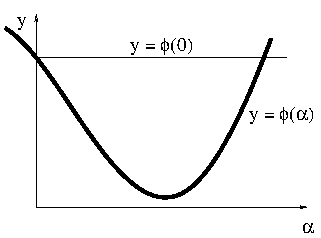
\includegraphics[width=0.53\linewidth]{assets/figures/fig-2-1.pdf}
\setcounter{figure}{0}
\caption{目标函数沿搜索直线的变化。}\label{fig:2.1}
\end{figure}

由于 $\mathbf{h}$ 是下降方向，故有
\[
  \varphi'(0)=\mathbf{h}^{\T}\mathbf{F}'(\mathbf{x})<0,
\]
这表明，如果 $\alpha$ 充分小，就能满足下降条件~(2.1)，它等价于
\[
  \varphi(\alpha)<\varphi(0).
\]
通常会给定一个 $\alpha$ 的初始猜测值，例如牛顿法中的 $\alpha=1$。
图~2.1~说明可能出现三种不同的情况：
\begin{enumerate}[label=\arabic*$^{\circ}$,leftmargin=2.4em]
  \item $\alpha$ 很小，因而目标函数值的下降量很小。应增大 $\alpha$。
  \item $\alpha$ 太大：$\varphi(\alpha)\geq\varphi(0)$。应减小 $\alpha$，
        以满足下降条件~(2.1)。
  \item $\alpha$ 接近 $\varphi(\alpha)$ 的极小点\footnote{更准确地说，是 $\varphi$
        的第一个局部极小点。如果把 $\alpha$ 增大到图~2.1~所示区间之外，完全有可能
        接近 $F$ 的另一个局部极小点。}。接受这一 $\alpha$ 值。
\end{enumerate}

\sourcepage{11}
\emph{精确线搜索}是一个产生序列 $\alpha_1,\alpha_2,\ldots$ 的迭代过程。
其目的是找到~(2.7) 所定义的真正极小点 $\alpha_{\mathrm e}$，当迭代值
$\alpha_{\mathrm s}$ 满足
\[
  |\varphi'(\alpha_{\mathrm s})|\leq\tau\,|\varphi'(0)|
\]
时，算法停止，其中 $\tau$ 是一个较小的正数。迭代中，可以根据已计算的值
\[
  \varphi(\alpha_k)=F(\mathbf{x}+\alpha_k\mathbf{h})
  \qquad\text{和}\qquad
  \varphi'(\alpha_k)=\mathbf{h}^{\T}\mathbf{F}'(\mathbf{x}+\alpha_k\mathbf{h})
\]
来近似 $\varphi(\alpha)$ 的变化。详见 Frandsen 等（2004）第~2.5--2.6~节。

精确线搜索可能浪费很多计算时间：当 $\mathbf{x}$ 远离 $\mathbf{x}^{\ast}$ 时，搜索方向
$\mathbf{h}$ 可能与 $\mathbf{x}^{\ast}-\mathbf{x}$ 的方向相差甚远，没有必要非常精确地找到
$\varphi$ 的真正极小值。这就是所谓的\emph{非精确线搜索}的出发点：只要一个
$\alpha$ 值不属于上面列出的第~$1^{\circ}$ 或第~$2^{\circ}$ 种情况，就可以接受它。
我们采用比下降条件~(2.1) 更严格的条件，即
\begin{equation}
  \varphi(\alpha_{\mathrm s})
  \leq\varphi(0)+\gamma_1\cdot\varphi'(0)\cdot\alpha
  \qquad\text{其中 }0<\gamma_1<1.
  \tag{2.13a}\label{eq:2.13a}
\end{equation}
这保证了不会出现第~$2^{\circ}$ 种情况。第~$1^{\circ}$ 种情况对应于点
$(\alpha,\varphi(\alpha))$ 太接近起点处的切线，因此再补充条件
\begin{equation}
  \varphi'(\alpha_{\mathrm s})\geq\gamma_2\cdot\varphi'(0)
  \qquad\text{其中 }\gamma_1<\gamma_2<1.
  \tag{2.13b}\label{eq:2.13b}
\end{equation}
如果 $\alpha$ 的初始猜测值满足这两个准则，我们就接受它作为 $\alpha_{\mathrm s}$。
否则，必须按照前述精确线搜索的方式迭代。详见 Frandsen 等（2004）第~2.5~节。

\section{信赖域法与阻尼法}
假设有一个模型 $L$，描述 $F$ 在当前迭代点 $\mathbf{x}$ 邻域内的性质，
\begin{equation}
  F(\mathbf{x}+\mathbf{h})\simeq L(\mathbf{h})
  \equiv F(\mathbf{x})+\mathbf{h}^{\T}\mathbf{c}
       +\tfrac12\mathbf{h}^{\T}\mathbf{B}\mathbf{h},
  \tag{2.14}\label{eq:2.14}
\end{equation}

\sourcepage{12}
其中 $\mathbf{c}\in\R^n$，矩阵 $\mathbf{B}\in\R^{n\times n}$ 是对称的。本节的基本思想
可以推广到其他形式的模型，但本讲义只需要~(2.14) 所给形式的 $L$。通常，这一模型是
$F$ 在 $\mathbf{x}$ 附近的二阶泰勒展开，例如~(1.4a) 右端的前三项；$L(\mathbf{h})$ 也可以是
这一展开的近似。一般而言，只有 $\mathbf{h}$ 充分小时，这样的模型才是好的近似。

下面介绍两种在确定步子 $\mathbf{h}$ 时考虑这一点的方法。所得步子沿下降方向，并可在
算法~2.4~中取 $\alpha=1$ 使用。

在\emph{信赖域法}中，我们假设已知一个正数 $\Delta$，使模型在以 $\mathbf{x}$ 为中心、
半径为 $\Delta$ 的球内足够准确，并按下式确定步子：
\begin{equation}
  \mathbf{h}=\mathbf{h}_{\mathrm{tr}}
  \equiv\operatorname*{argmin}_{\norm{\mathbf{h}}\leq\Delta}\{L(\mathbf{h})\}.
  \tag{2.15}\label{eq:2.15}
\end{equation}

在\emph{阻尼法}中，步子由下式确定：
\begin{equation}
  \mathbf{h}=\mathbf{h}_{\mathrm{dm}}
  \equiv\operatorname*{argmin}_{\mathbf{h}}
  \{L(\mathbf{h})+\tfrac12\mu\mathbf{h}^{\T}\mathbf{h}\},
  \tag{2.16}\label{eq:2.16}
\end{equation}
其中\emph{阻尼参数} $\mu\geq0$。可以看出，附加项
$\tfrac12\mu\mathbf{h}^{\T}\mathbf{h}=\tfrac12\mu\norm{\mathbf{h}}^2$ 对较大的步子施加惩罚。

基于上述任一方法，算法~2.4~的核心部分都具有如下形式：
\begin{equation}
\begin{aligned}
  &\text{由~(2.15) 或~(2.16) 计算 }\mathbf{h}\\
  &\textbf{if}\quad F(\mathbf{x}+\mathbf{h})<F(\mathbf{x})\\
  &\qquad\mathbf{x}:=\mathbf{x}+\mathbf{h}\\
  &\text{更新 }\Delta\text{ 或 }\mu
\end{aligned}
\tag{2.17}\label{eq:2.17}
\end{equation}
若步子 $\mathbf{h}$ 满足下降条件~(2.1)，这就相当于 $\alpha=1$。否则，$\alpha=0$，
即不移动\footnote{这两类方法也有包含真正线搜索的版本：寻找 $F$ 值更小的点
$\mathbf{x}+\alpha\mathbf{h}$，并利用线搜索中获得的信息更新 $\Delta$ 或 $\mu$。
对于许多问题，这类版本采用的迭代步数较少，但累计函数求值次数更多。}。
不过，我们不会停滞在
\sourcepage{13}
$\mathbf{x}$ 处（除非 $\mathbf{x}=\mathbf{x}^{\ast}$）：通过适当地修改 $\Delta$ 或 $\mu$，
我们力求在下一次迭代中得到更好的结果。

由于假定 $\mathbf{h}$ 充分小时 $L(\mathbf{h})$ 是 $F(\mathbf{x}+\mathbf{h})$ 的良好近似，
所以一步失败的原因是 $\mathbf{h}$ 太大，应当缩小。另外，如果这一步被接受，那么从新的
迭代点出发也许可以采用更大的步子，从而减少到达 $\mathbf{x}^{\ast}$ 所需的步数。

对于已经计算出的步子，可以用所谓的\emph{增益比}来评价模型的质量，
\begin{equation}
  \varrho=\frac{F(\mathbf{x})-F(\mathbf{x}+\mathbf{h})}{L(\mathbf{0})-L(\mathbf{h})},
  \tag{2.18}\label{eq:2.18}
\end{equation}
即函数值的实际下降量与预测下降量之比。按构造，分母为正；如果这一步没有沿下降方向移动，
分子为负，此时步子太大，应当缩小。

在信赖域法中，我们通过半径 $\Delta$ 的大小来控制步长。下面的更新策略被广泛采用：
\begin{equation}
\begin{aligned}
  &\textbf{if}\quad\varrho<0.25\\
  &\qquad\Delta:=\Delta/2\\
  &\textbf{elseif}\quad\varrho>0.75\\
  &\qquad\Delta:=\max\{\Delta,3*\norm{\mathbf{h}}\}
\end{aligned}
\tag{2.19}\label{eq:2.19}
\end{equation}
因此，如果 $\varrho<\tfrac14$，就决定采用较小的步子；而 $\varrho>\tfrac34$
则表明可能可以采用更大的步子。信赖域算法对阈值 $0.25$ 和 $0.75$、除数 $p_1=2$
或乘数 $p_2=3$ 的小幅改变并不敏感，但必须恰当地选择 $p_1$ 和 $p_2$，使
$\Delta$ 值不会发生振荡。

在阻尼法中，较小的 $\varrho$ 值表明应增大阻尼因子，从而加重对大步子的惩罚。
较大的 $\varrho$ 值则表明，对于计算出的 $\mathbf{h}$，$L(\mathbf{h})$ 是
$F(\mathbf{x}+\mathbf{h})$ 的良好近似，此时可减小阻尼。下面这个与~(2.19) 类似的策略
被广泛使用，它最初由 Marquardt（1963）提出，

\sourcepage{14}
\begin{equation}
\begin{aligned}
  &\textbf{if}\quad\varrho<0.25\\
  &\qquad\mu:=\mu*2\\
  &\textbf{elseif}\quad\varrho>0.75\\
  &\qquad\mu:=\mu/3
\end{aligned}
\tag{2.20}\label{eq:2.20}
\end{equation}
同样，方法对阈值 $0.25$、$0.75$ 或数值 $p_1=2$、$p_2=3$ 的小幅改变并不敏感，
但必须恰当地选择 $p_1$ 和 $p_2$，使 $\mu$ 值不会发生振荡。经验表明，跨越阈值
$0.25$ 和 $0.75$ 时的不连续变化可能引起“抖动”（第~\pageref{src:27}~页的
例~3.7~对此有说明），从而减慢收敛。我们在 Nielsen（1999）中证明，以下策略的表现
通常优于~(2.20)：
\begin{equation}
\begin{aligned}
  &\textbf{if}\quad\varrho>0\\
  &\qquad\mu:=\mu*\max\{\tfrac13,1-(2\varrho-1)^3\};\quad\nu:=2\\
  &\textbf{else}\\
  &\qquad\mu:=\mu*\nu;\quad\nu:=2*\nu
\end{aligned}
\tag{2.21}\label{eq:2.21}
\end{equation}
因子 $\nu$ 初始化为 $\nu=2$。注意，连续多次失败会使 $\mu$ 值迅速增大。
图~2.2~展示了这两个更新公式。

\begin{figure}[H]
\centering
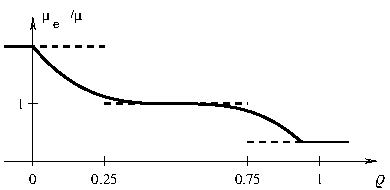
\includegraphics[width=0.64\linewidth]{assets/figures/fig-2-2.pdf}
\setcounter{figure}{1}
\caption{按~(2.21) 且取 $\nu=2$ 更新 $\mu$（实线），以及 Marquardt 的策略~(2.20)（虚线）。}
\label{fig:2.2}
\end{figure}

\subsection{迭代步的计算}
在阻尼法中，步子通过求函数
\[
  \psi_{\mu}(\mathbf{h})=L(\mathbf{h})+\tfrac12\mu\mathbf{h}^{\T}\mathbf{h}
\]
的驻点来计算。

\sourcepage{15}
这意味着 $\mathbf{h}_{\mathrm{dm}}$ 是方程
\[
  \psi'_{\mu}(\mathbf{h})=\mathbf{L}'(\mathbf{h})+\mu\mathbf{h}=\mathbf{0}
\]
的一个解。由~(2.14) 中 $L(\mathbf{h})$ 的定义可知，这等价于
\begin{equation}
  (\mathbf{B}+\mu\mathbf{I})\mathbf{h}_{\mathrm{dm}}=-\mathbf{c},
  \tag{2.22}\label{eq:2.22}
\end{equation}
其中 $\mathbf{I}$ 为单位矩阵。如果 $\mu$ 充分大，对称矩阵 $\mathbf{B}+\mu\mathbf{I}$ 就是
正定的（附录~A~中有证明），于是由定理~1.8~可知 $\mathbf{h}_{\mathrm{dm}}$ 是 $L$ 的极小点。

\begin{example}{2.1}
在\emph{阻尼牛顿法}中，模型 $L(\mathbf{h})$ 由 $\mathbf{c}=\mathbf{F}'(\mathbf{x})$ 和
$\mathbf{B}=\mathbf{F}''(\mathbf{x})$ 给出，因而~(2.22) 化为
\[
  \bigl(\mathbf{F}''(\mathbf{x})+\mu\mathbf{I}\bigr)\mathbf{h}_{\mathrm{dn}}=-\mathbf{F}'(\mathbf{x}).
\]
$\mathbf{h}_{\mathrm{dn}}$ 称为阻尼牛顿步。如果 $\mu$ 很大，则
\[
  \mathbf{h}_{\mathrm{dn}}\simeq-\frac{1}{\mu}\mathbf{F}'(\mathbf{x}),
\]
即沿接近最速下降方向的方向迈出一小步。另一方面，如果 $\mu$ 很小，
$\mathbf{h}_{\mathrm{dn}}$ 就接近牛顿步 $\mathbf{h}_{\mathrm n}$。因此，可以把阻尼牛顿法
看作最速下降法与牛顿法的混合。
\end{example}

我们将在第~3.2~节重新讨论阻尼法。

在信赖域法中，步子 $\mathbf{h}_{\mathrm{tr}}$ 是一个\emph{约束优化问题}的解，
\begin{equation}
\begin{aligned}
  &\text{最小化}\quad L(\mathbf{h})\\
  &\text{约束条件}\quad\mathbf{h}^{\T}\mathbf{h}\leq\Delta^2.
\end{aligned}
\tag{2.23}\label{eq:2.23}
\end{equation}
详细讨论这个问题超出了本讲义的范围（见 Madsen 等（2004），或 Nocedal 与
Wright（1999）第~4.1~节）。这里只提及它的几个性质。

如果~(2.14) 中的矩阵 $\mathbf{B}$ 正定，那么 $L$ 的无约束极小点是方程
\sourcepage{16}
\[
  \mathbf{B}\mathbf{h}=-\mathbf{c}
\]
的解；如果这个解足够小（即满足 $\mathbf{h}^{\T}\mathbf{h}\leq\Delta^2$），它就是所需的步子
$\mathbf{h}_{\mathrm{tr}}$。否则，约束是有效的，问题也更复杂。与第~\pageref{src:11}~页
所用论证类似，可以看出，我们不必计算~(2.23) 的真正解；第~3.3~节和第~3.4~节将介绍
两种计算 $\mathbf{h}_{\mathrm{tr}}$ 近似值的方法。

最后，在 $\mathbf{B}$ 正定的情形下，介绍阻尼法与信赖域法的两个相似之处。
当无约束极小点位于信赖域之外时，可以证明（Madsen 等（2004）的定理~2.11），
存在一个 $\lambda>0$，使得
\begin{equation}
  \mathbf{B}\mathbf{h}_{\mathrm{tr}}+\mathbf{c}=-\lambda\mathbf{h}_{\mathrm{tr}}.
  \tag{2.24a}\label{eq:2.24a}
\end{equation}
将这个方程移项，再与~(2.22) 比较，可见 $\mathbf{h}_{\mathrm{tr}}$ 与采用阻尼参数
$\mu=\lambda$ 算出的阻尼步 $\mathbf{h}_{\mathrm{dm}}$ 完全相同。另一方面，也可以证明
（Frandsen 等（2004）的定理~5.11），如果给定 $\mu\geq0$ 并计算出
$\mathbf{h}_{\mathrm{dm}}$，则
\begin{equation}
  \mathbf{h}_{\mathrm{dm}}
  =\operatorname*{argmin}_{\norm{\mathbf{h}}\leq\norm{\mathbf{h}_{\mathrm{dm}}}}
      \{L(\mathbf{h})\},
  \tag{2.24b}\label{eq:2.24b}
\end{equation}
即 $\mathbf{h}_{\mathrm{dm}}$ 等于信赖域半径 $\Delta=\norm{\mathbf{h}_{\mathrm{dm}}}$
所对应的 $\mathbf{h}_{\mathrm{tr}}$。因此，这两类方法密切相关，但对于给出相同步子的
$\Delta$ 值与 $\mu$ 值，它们之间并不存在简单的联系公式。
